\PassOptionsToPackage{unicode}{hyperref}
\documentclass[aspectratio=169, 9pt, bibliography=totoc]{beamer}

\usepackage{polyglossia}
\setmainlanguage{german}
\usepackage{csquotes}
\usepackage{scrhack}
\usepackage{amsmath}
\usepackage{amssymb}
\usepackage{mathtools}
\usepackage{unicode-math}
\usepackage[
  locale=DE,
  separate-uncertainty=true,
  per-mode=symbol-or-fraction,
]{siunitx}
\usepackage{xfrac}
\usepackage{float}
\floatplacement{figure}{htbp}
\floatplacement{table}{htbp}
\usepackage{pgfplotstable}
\usepackage{array}
\usepackage{subcaption}
\usepackage{graphicx}
\usepackage{booktabs}
\usepackage{microtype}
\usepackage{hyperref}
\usepackage{bookmark}
\usepackage[backend=biber]{biblatex}
\addbibresource{lit.bib}
\usetheme[
  %  showtotalframes,
]{tudo}
\unimathsetup{
  math-style=ISO,
  bold-style=ISO,
  nabla=upright,
  partial=upright,
  mathrm=sym,
  warnings-off={
    mathtools-colon,
    mathtools-overbracket,
  },
}


\title{Tarnung}
\author[C.~Beckmann]{Christian Beckmann}
\institute[Seminar Moderne Optik]{Seminar Moderne Optik}
\titlegraphic{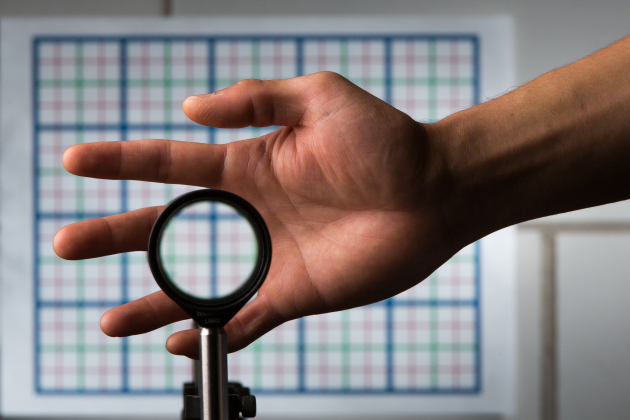
\includegraphics[height=0.6\textheight]{images/hand-cloak.jpg}}
\date{08. Mai 2019}
%\newcommand \matrize[1]{\underline{\underline{#1}}}
\begin{document}

\maketitle

\begin{frame}{Themen\"ubersicht}
  \tableofcontents
\end{frame}

\section{Definition des Begriffes}

\begin{frame}{Der Begriff \textit{tarnen}}
  Definition des Duden:
  \begin{block}{{\centering tar - nen}}
    jemanden, etwas vor dem Erkannt-, Gesehenwerden sch\"utzen,
    indem man es verh\"ullt oder der Umgebung angleicht
  \end{block}
\end{frame}

\section{Beispiele}
\begin{frame}{Ein Blick in die Natur.}
  \begin{figure}
    \centering
    \caption{Ein \textit{getarnter} Luchs im Dortmunder Zoo.}
    \includegraphics[width=0.6\textwidth]{images/luchs-do.JPG}
  \end{figure}
\end{frame}

\begin{frame}{Funktioniert das auch f\"ur Menschen?}
  \begin{figure}
    \centering
    \caption{Der Chinesische K\"unstler Liu Bolin tarnt sich. \cite{humanhide}}
    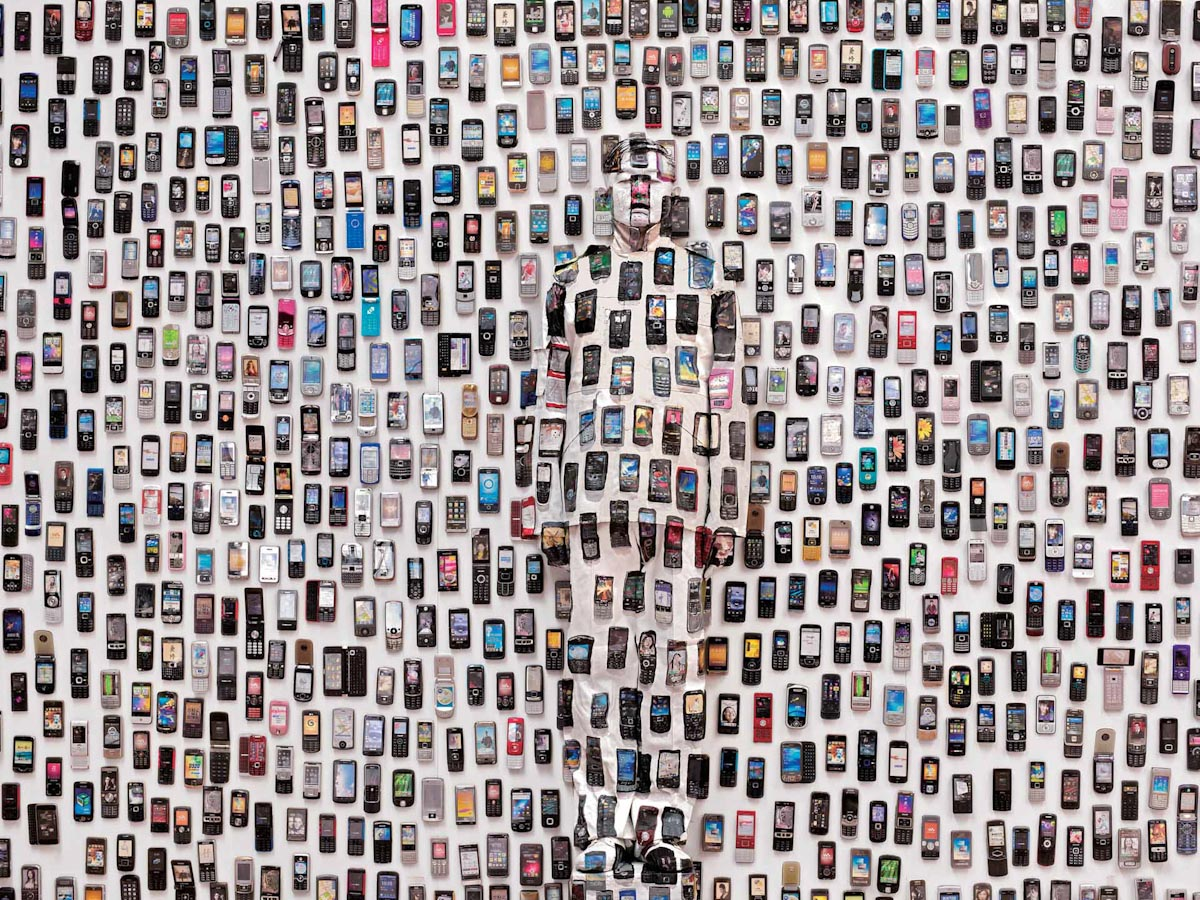
\includegraphics[height=0.8\textheight]{images/liubolin.jpg}
  \end{figure}
\end{frame}

\begin{frame}{Dynamisch statt statisch}
  Im Radarwellenbereich, $λ = \SI{10}{\centi\meter}$, können Flugzeuge getarnt werden.
  Der B-2 Spirit Tarnkappenbomer hat eine Radarreflexion eines kleinen Vogels.
  \begin{figure}
    \centering
    \begin{subfigure}{0.48\textwidth}
      \centering
      \caption{Eine Aufnahme der B-2 Spirit (US-Luftwaffe). \cite{b2spirit}}
      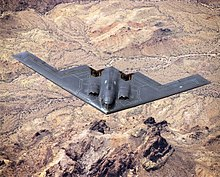
\includegraphics[width=0.7\textwidth]{images/b2spirit.jpg}
    \end{subfigure}
    \begin{subfigure}{0.48\textwidth}
      \centering
      \caption{Ein Bild eines Spatzen zum Vergleich. \cite{spatz}}
      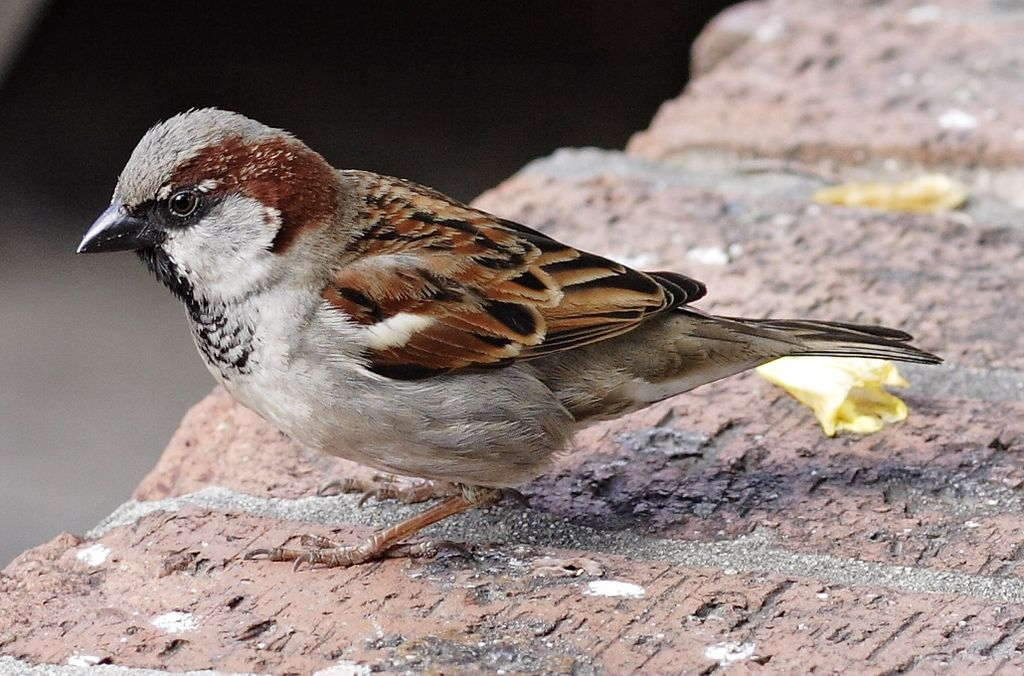
\includegraphics[width=0.7\textwidth]{images/spatz.jpg}
    \end{subfigure}
  \end{figure}
\end{frame}

\begin{frame}{Sichtbarer Bereich}
  \begin{columns}
    \begin{column}{0.48\textwidth}
      \begin{figure}
        \centering
        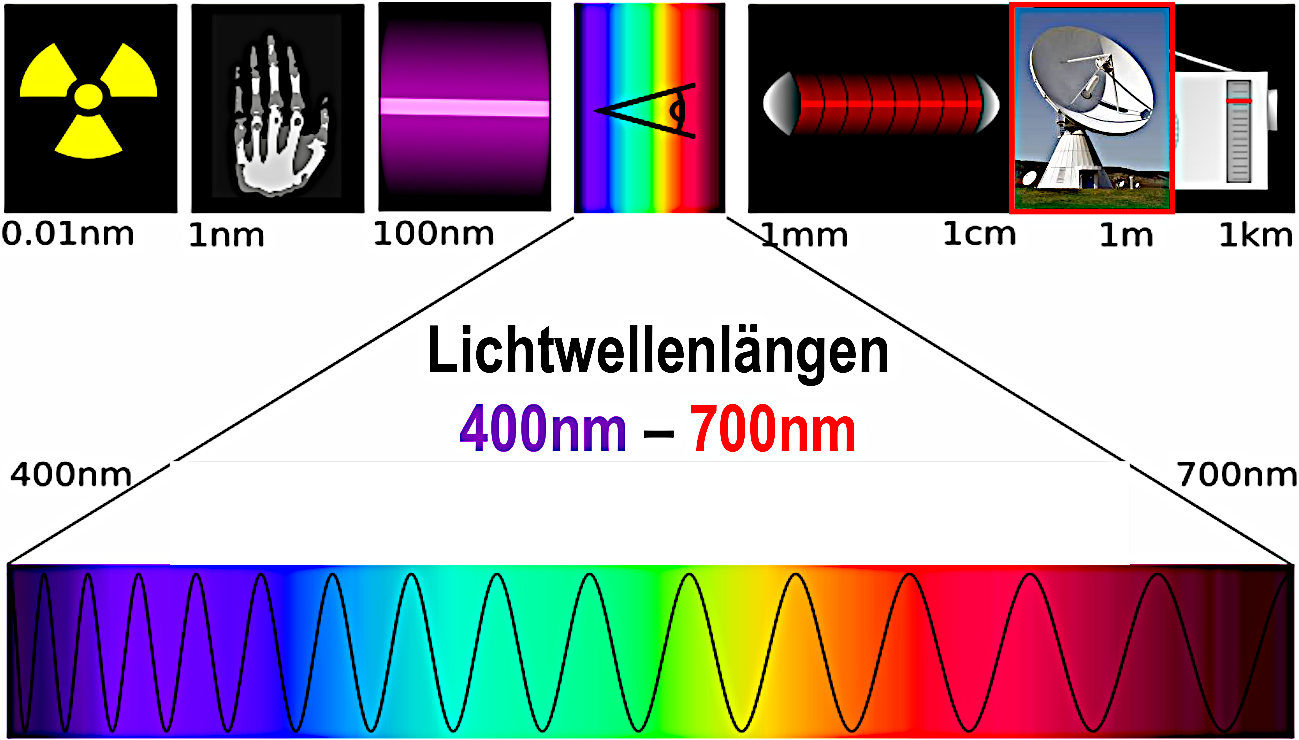
\includegraphics[width=\textwidth]{images/wellenbereich.png}
        \caption{Das Spektrum elektromagnetischer Wellen.}
      \end{figure}
    \end{column}
    \begin{column}{0.48\textwidth}
      Im optischen Bereich ist ein Objekt mit hoher Absorption leicht zu erkennen,
      da der Hintergrund nicht sichtbar ist. \\
      $\implies$ Das Licht muss um das Objekt herumgef\"uhrt werden.
    \end{column}
  \end{columns}
\end{frame}

\begin{frame}{Ablenkung von Licht}
  \begin{figure}
    \caption{Das schwarze Loch in Messier 87, \cite{m87}}
    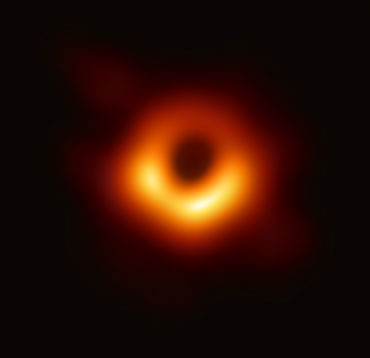
\includegraphics[height=0.8\textheight]{images/m87.jpg}
  \end{figure}
\end{frame}

\section{Ein Beispiel zum rechnen und nachbauen}

\begin{frame}{Das System}
  \begin{figure}
    \caption{Eine Hand kann in das System gehalten werden und der Hintergrund ist weiterhin zu sehen.}
    \centering
    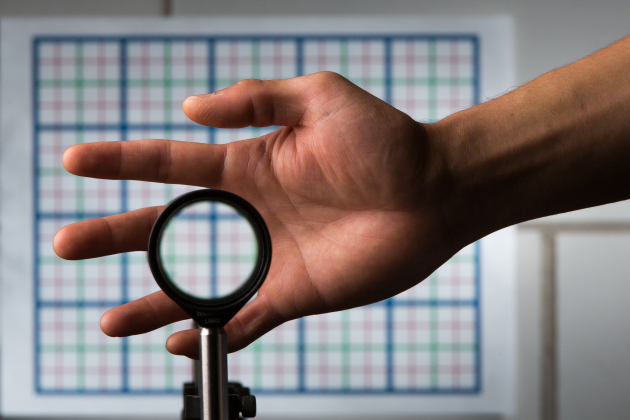
\includegraphics[height=0.6\textheight]{images/hand-cloak.jpg}
  \end{figure}
  Die folgenden Folien beziehen sich auf
  \href{https://www.rochester.edu/newscenter/watch-rochester-cloak-uses-ordinary-lenses-to-hide-objects-across-continuous-range-of-angles-70592/}{diese Veröffentlichung}
  von Howell und Choi der Universität Rochester aus dem Jahr 2014.
\end{frame}

\subsection{Einschub: Matrizenoptik}
\begin{frame}{Matrizenoptik}
  \begin{columns}
    \begin{column}{0.48\textwidth}
      \begin{figure}
        \centering
        \caption{Das System in Seitenansicht.}
        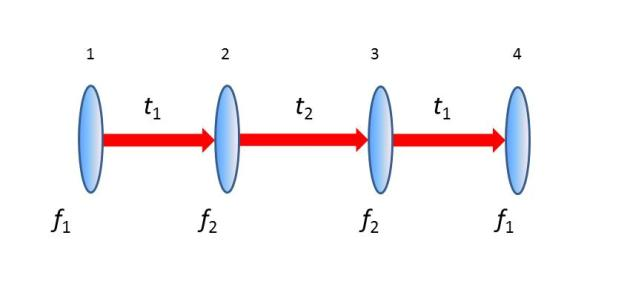
\includegraphics[width=\textwidth]{images/linsen.jpg}
      \end{figure}
    \end{column}
    \begin{column}{0.48\textwidth}
      D\"unne Linse
      \begin{align*}
        F_i &=
        \begin{pmatrix}
          1 & 0 \\
          -\frac{1}{f_i} & 1 \\
        \end{pmatrix}
        \intertext{Translation}
        T_i &=
        \begin{pmatrix}
          1 & t_i \\
          0 & 1 \\
        \end{pmatrix}
      \end{align*}
    \end{column}
  \end{columns}
\end{frame}

\begin{frame}{Matrizenoptik - Grundlagen}
  Annahmen der Matrizenoptik:
  \begin{enumerate}
    \item $λ\:<\!<$ alle Abmessungen des Systems $\to$ geometrische Optik
    \item axialsymmetrische Strahlen
    \item achsennahe Strahlen: $\sin(α) \approx \tan(α) \approx α$
  \end{enumerate}
  \pause
  \begin{columns}
    \begin{column}{0.4\textwidth}
      Beschreibung der Strahlen durch
      \begin{align*}
        \text{Achsenabstand}\;&y \\
        \text{Steigung}\;&v
        \intertext{Betrachtung des Brechungsindizes $n$:}
        V &\coloneq nv \\
        t &\coloneq \frac{x}{n}
      \end{align*}
    \end{column}
    \begin{column}{0.58\textwidth}
      Translationsmatrix:
      \begin{align*}
        \begin{pmatrix} y_2 \\ v_2 \\ \end{pmatrix} =
        \begin{pmatrix} 1 & x \\ 0 & 1 \\ \end{pmatrix}
        \begin{pmatrix} y_1 \\ v_1 \\ \end{pmatrix}
        &\implies
        \begin{pmatrix} Y_2 \\ V_2 \\ \end{pmatrix} =
        \begin{pmatrix} 1 & t \\ 0 & 1 \\ \end{pmatrix}
        \begin{pmatrix} Y_1 \\ V_1 \\ \end{pmatrix}
        \intertext{Refraktionsmatrix (d\"unne Linsen):}
        R = \begin{pmatrix} 1 & 0 \\ -\frac{n_2-n_1}{r} & 1 \\ \end{pmatrix}
        &\implies \begin{pmatrix} 1 & 0 \\ -P & 1 \\ \end{pmatrix}
        = \begin{pmatrix} 1 & 0 \\ -\frac{1}{f} & 1 \\ \end{pmatrix} \\
        f &: \text{Brennweite}
      \end{align*}
    \end{column}
  \end{columns}
\end{frame}

\subsection{Diskussion des Systems}
\begin{frame}{Warum vier Linsen?}
  Eine Tarnkappe der L\"ange $L$ wird in der Matrizenoptik durch
  \begin{align*}
    M_\text{tarn} &=
    \begin{pmatrix}
      1 & L \\
      0 & 1 \\
    \end{pmatrix}
    =
    \begin{pmatrix}
      A & B \\
      C & D \\
    \end{pmatrix}
    \intertext{dargestellt. Eine Linse kann diese Bedingung nur erfüllen, wenn}
    M_{L=1} &=
    \begin{pmatrix}
      1 & 0 \\
      -\frac{1}{f_1} & 1 \\
    \end{pmatrix} = M_\text{tarn}
    \intertext{gilt, also}
    f_1 &\to \infty\:.
  \end{align*}
  Das entspricht einer Glasscheibe.
\end{frame}

\begin{frame}{Zwei Linsen}
  Die Gleichung f\"ur zwei Linsen lautet
  \begin{align*}
    M_{L=2} &= F_2\:T_1\:F_1 =
    \begin{pmatrix}
      1-\frac{t_1}{f_1} & t_1 \\
      -\frac{f_1+f_2-t_1}{f_1f_2} & 1-\frac{t_1}{f_2} \\
    \end{pmatrix}
    \stackrel{!}{=}
    \begin{pmatrix} A & B \\ C & D \\ \end{pmatrix} =
    \begin{pmatrix} 1 & L \\ 0 & 1 \\ \end{pmatrix}
    \intertext{Daraus folgt}
    \begin{drcases}
      t_1 = L = 0 \\
      f_1 \to \infty \\
      f_2 \to \infty
    \end{drcases}
    &=
    \begin{pmatrix}
      1 & 0 \\
      0 & 1 \\
    \end{pmatrix}
  \end{align*}
\end{frame}

\begin{frame}{Erweiterung auf drei Linsen}
  \begin{equation*}
    M_{L=3} = F_3\:T_2\:M_{L=2} = \frac{1}{f_2}
    \begin{pmatrix}
      \frac{f_1f_2-t_1f_2-t_2f_2-t_2f_1+t_1t_2}{f_1} & t_1f_2-t_1t_2+t_2f_2 \\
      -\frac{f_1f_2+f_2f_3-t_1f_2-t_2f_2+f_1f_3-t_1f_3-t_2f_1+t_1t_2}{f_1f_3}
      & \frac{f_2f_3-t_1f_3-t_1f_2-t_2f_2+t_1t_2}{f_3} \\
    \end{pmatrix}
    \stackrel{!}{=}
    \begin{pmatrix} A & B \\ C & D \\ \end{pmatrix} =
    \begin{pmatrix} 1 & L \\ 0 & 1 \\ \end{pmatrix}
  \end{equation*}
  Es ergeben sich durch die Bedingungen einer Tarnkappe:
  \begin{columns}
    \begin{column}{0.32\textwidth}
      \begin{align*}
        C &= 0 \\
        f_2 &= -\frac{(f_3-t_2)(f_1-t_1)}{f_1+f_3-t_1-t_2}
      \end{align*}
    \end{column}
    \begin{column}{0.32\textwidth}
      \begin{align*}
        B &= L = t_1 + t_2 - \frac{t_1t_2}{f_2} \\
        0 &= t_1 t_2 \frac{f_1+f_3-t_1-t_2}{(f_3-t_2)(f_1-t_1)}\\
        &\implies t_1 = 0\;\text{v}\;t_2 = 0 \\
        &\text{v}\;f_1+f_3-t_1-t_2 = 0
      \end{align*}
    \end{column}
    \begin{column}{0.32\textwidth}
      \begin{align*}
        f_1 &= f_3 \;\wedge\; t_1 = t_2 \\
        f_2 &= \frac{t_1-f_1}{2}
      \end{align*}
      mit $f_1>\!>t_1$ $\implies$ Tarnkappe
    \end{column}
  \end{columns}
\end{frame}

\begin{frame}{Schließlich das System mit allen vier Linsen}
  \begin{columns}
    \begin{column}{0.48\textwidth}
      \begin{align*}
        f_1 &= f_4 \\
        f_2 &= f_3
      \end{align*}
    \end{column}
  \end{columns}  
\end{frame}

\section{Weitere Beispielsysteme}
\begin{frame}{Weitere Beispiele der Arbeitsgruppe Howell}
    In einer weiteren Ver\"offentlichung \cite{rochester2} sind andere kosteng\"unstige Beispiele dargestellt.
    \begin{figure}
        \centering
        \begin{subfigure}{0.48\textwidth}
            \centering
            \caption{Skizze des Systems.}
            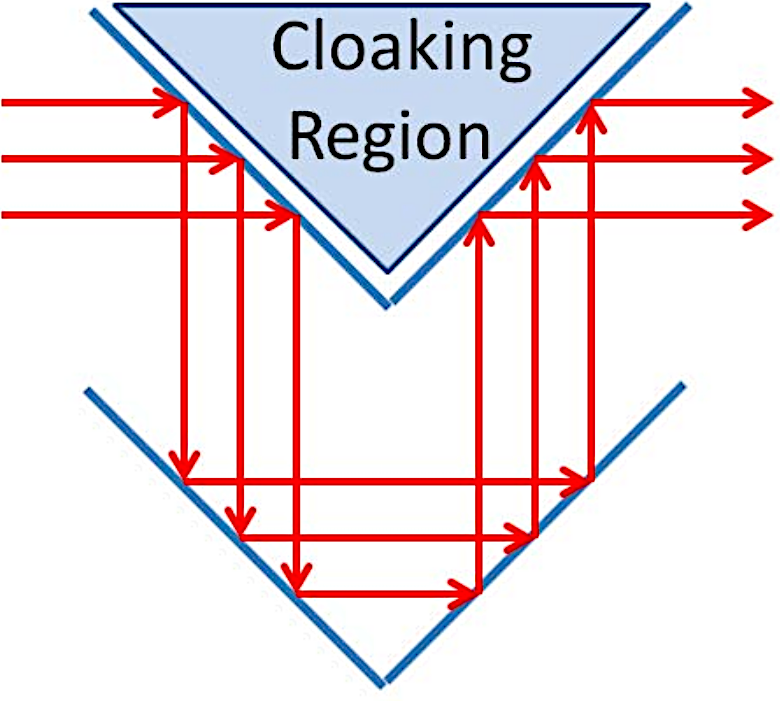
\includegraphics[height=0.6\textheight]{images/spiegel-skizze.png}
        \end{subfigure}
        \begin{subfigure}{0.48\textwidth}
            \centering
            \caption{Frontansicht des Systems.}
            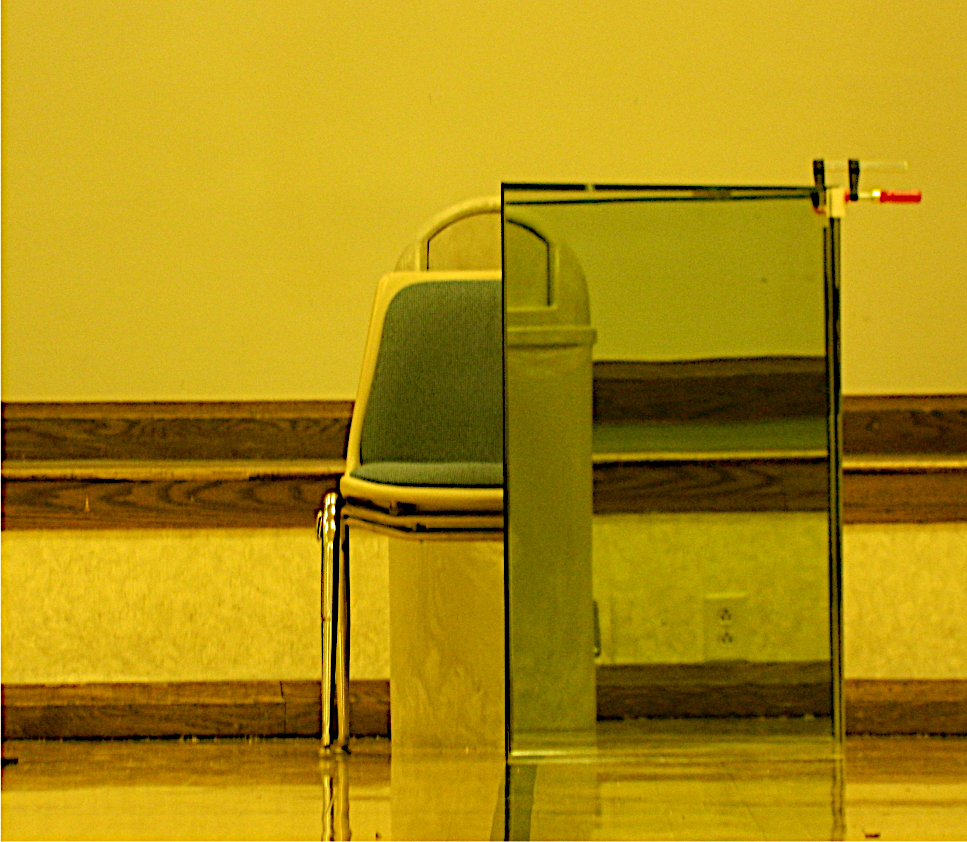
\includegraphics[height=0.6\textheight]{images/spiegel-vorne.png}
        \end{subfigure}
        \caption{Eine Tarnung aus Spiegeln.}
    \end{figure}
\end{frame}

\begin{frame}{Ein weiteres 'Linsensystem'}
    \begin{columns}
        \begin{column}{0.48\textwidth}
            \begin{figure}
                \centering
                \begin{subfigure}{\textwidth}
                    \centering
                    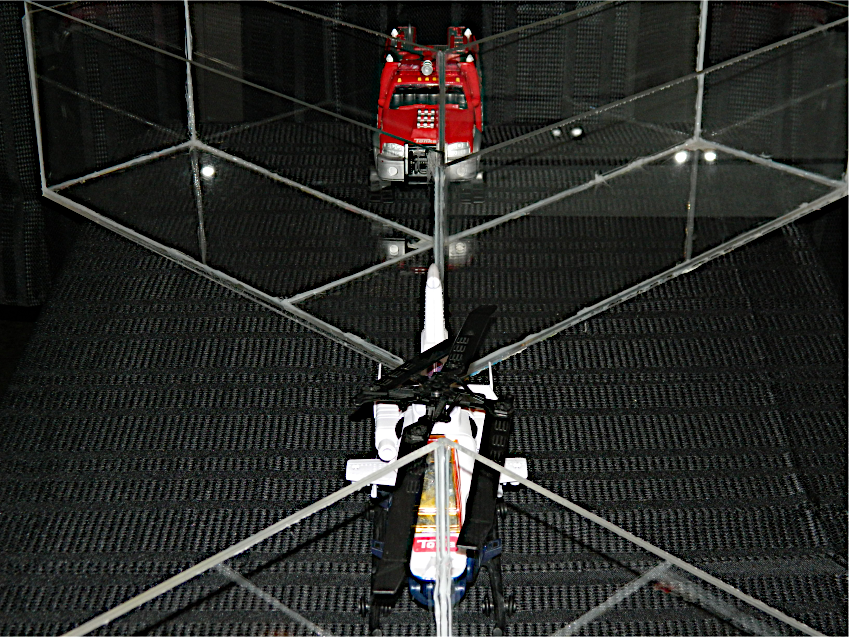
\includegraphics[height=0.4\textheight]{images/fresnel-oben.png}
                \end{subfigure}
                \begin{subfigure}{\textwidth}
                    \centering
                    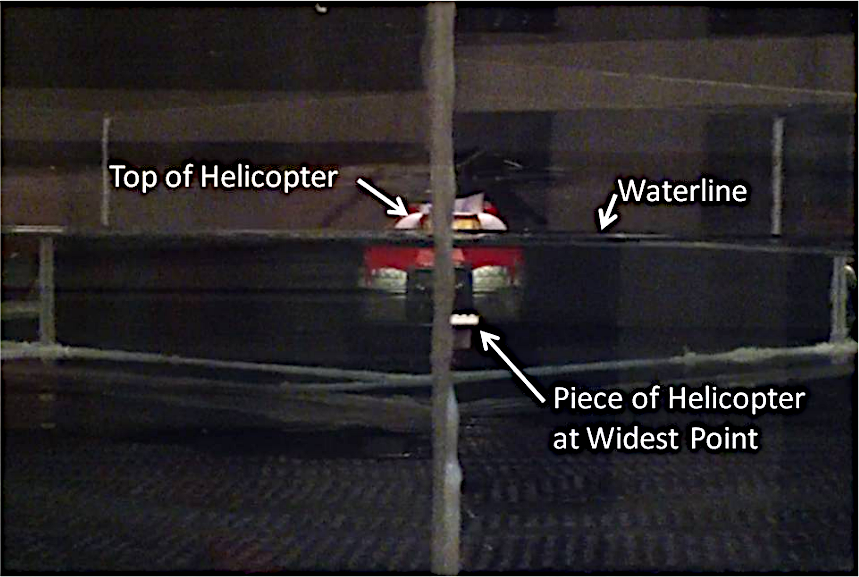
\includegraphics[height=0.4\textheight]{images/fresnel-vorne.png}
                \end{subfigure}
                \caption{Eine Tarnung mit Wasser.}
            \end{figure}
        \end{column}
        \begin{column}{0.48\textwidth}
            \begin{figure}
                \centering
                \caption{Skizze des Systems}
                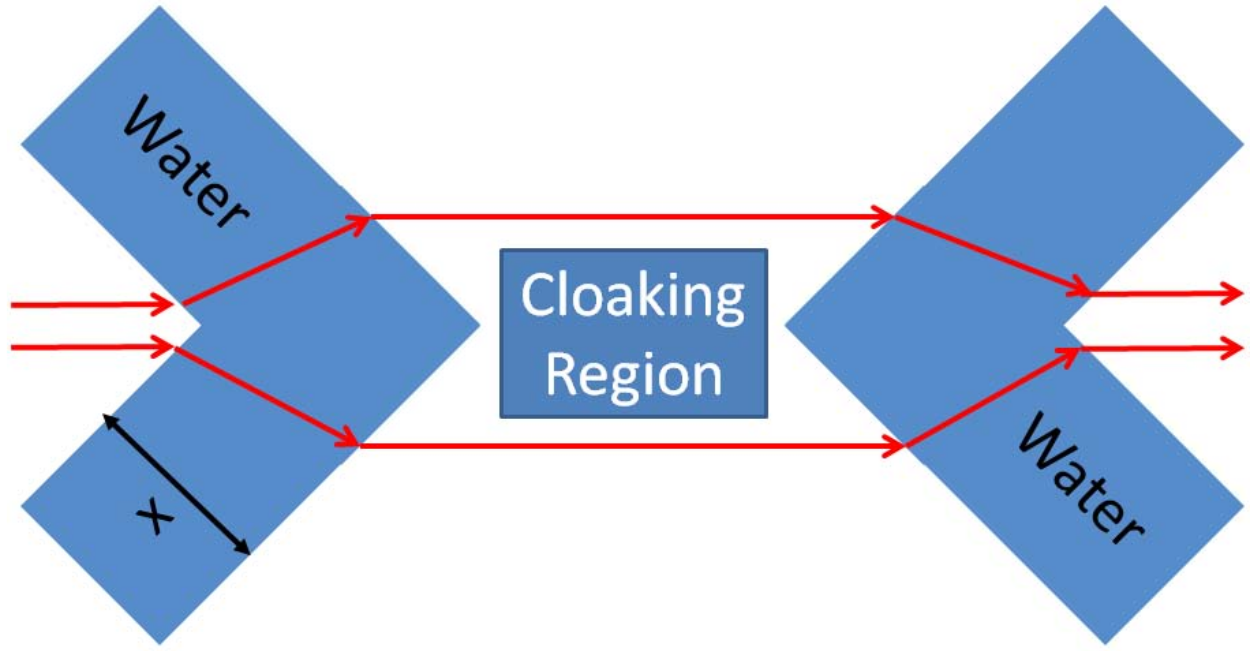
\includegraphics[height=0.3\textheight]{images/fresnel-skizze.png}
            \end{figure}
        \end{column}
    \end{columns}
\end{frame}


\begin{frame}{Zusammenfassung}
  \begin{itemize}
    \item Tarnung von Gegenständen im sichtbaren Bereich möglich
    \item tarnen der Tarnung ist schwierig
    \item $\SI{360}{\degree}$-Tarnung ist so nicht m\"oglich
  \end{itemize}
\end{frame}

\section{Literaturverzeichnis}
\begin{frame}
	\printbibliography
\end{frame}

\end{document}
